This section describes the development phase of our project. The development was started around the end of the 
needfinding phase once the team had a clear vision on the problems we were about to address and the solutions to get 
over those.

\subsection{Proposal}
% what do we propose? 
Analyzing the identified needs, our team had several ideas on how to overcome the challenges. We critically analyzed 
multiple ideas, compared them to one another, discussed the potential challenges and decided what to include in or 
exclude from our development project. 

We decided to focus our project towards developing a facilitator tool towards more interactive, fun and regular break 
habits. This proposal aims to 
\begin{itemize}
	\item be applicable in any office environment,
	\item enhance relationship between office workers,
 	\item enhance the atmosphere in the office.
\end{itemize}

By regular breaks spent with colleagues, the interaction in the environment increases, therefore people get to known, 
social relationships enhance. This yields in better atmosphere and therefore better productivity among colleagues. On 
top of that, the solution will help to avoid long, breakless work hours and therefore enhance the well being of office 
workers. 

We propose a software, which tracks the activity of an office worker while he/she is sitting at the desk working. The 
software analyzes the activity of the person and identifies a need for a break to be taken. This can be done based on 
time spent sitting, actively working on a task, computer keyboard activity and so on. The sitting position may be 
determined for instance by placing pressure sensors to the person's chair and keeping track how long pressure is 
pressed on the chair's plate. For the time being, the software is scaled down to use a built-in timer (also known as 
the Pomodoro technique \footnote{\url{https://en.wikipedia.org/wiki/Pomodoro_Technique}}) to schedule breaks. 

An extension to this data, it would be possible to track signals of the person (e.g. heart rate or pulse) to determine 
how "aware" he/she is and suggest the need for a break based on this data stream. This point out of the scope of this 
study, however would be interesting to think about in further research. 

\subsection{Project planning and tooling}
Right before jumping into the development, the roles of the team members were chosen, the available resources were 
considered and our availability was analyzed. We discussed how individuals can contribute to the final outcome of the 
project, how we can use our tutors' resources, what the main milestones in the project are and how much time can the 
team members dedicate to this project. 

The Gantt chart on Figure \ref{gantt-chart} summarizes the project's timeline, with the main milestones and 
activities. The purple lines mark the scheduled time for the activity, while the orange lines mark the time frame in 
which an activity was executed, but not originally planned.
 
\begin{figure}[h] 
		\begin{center}
			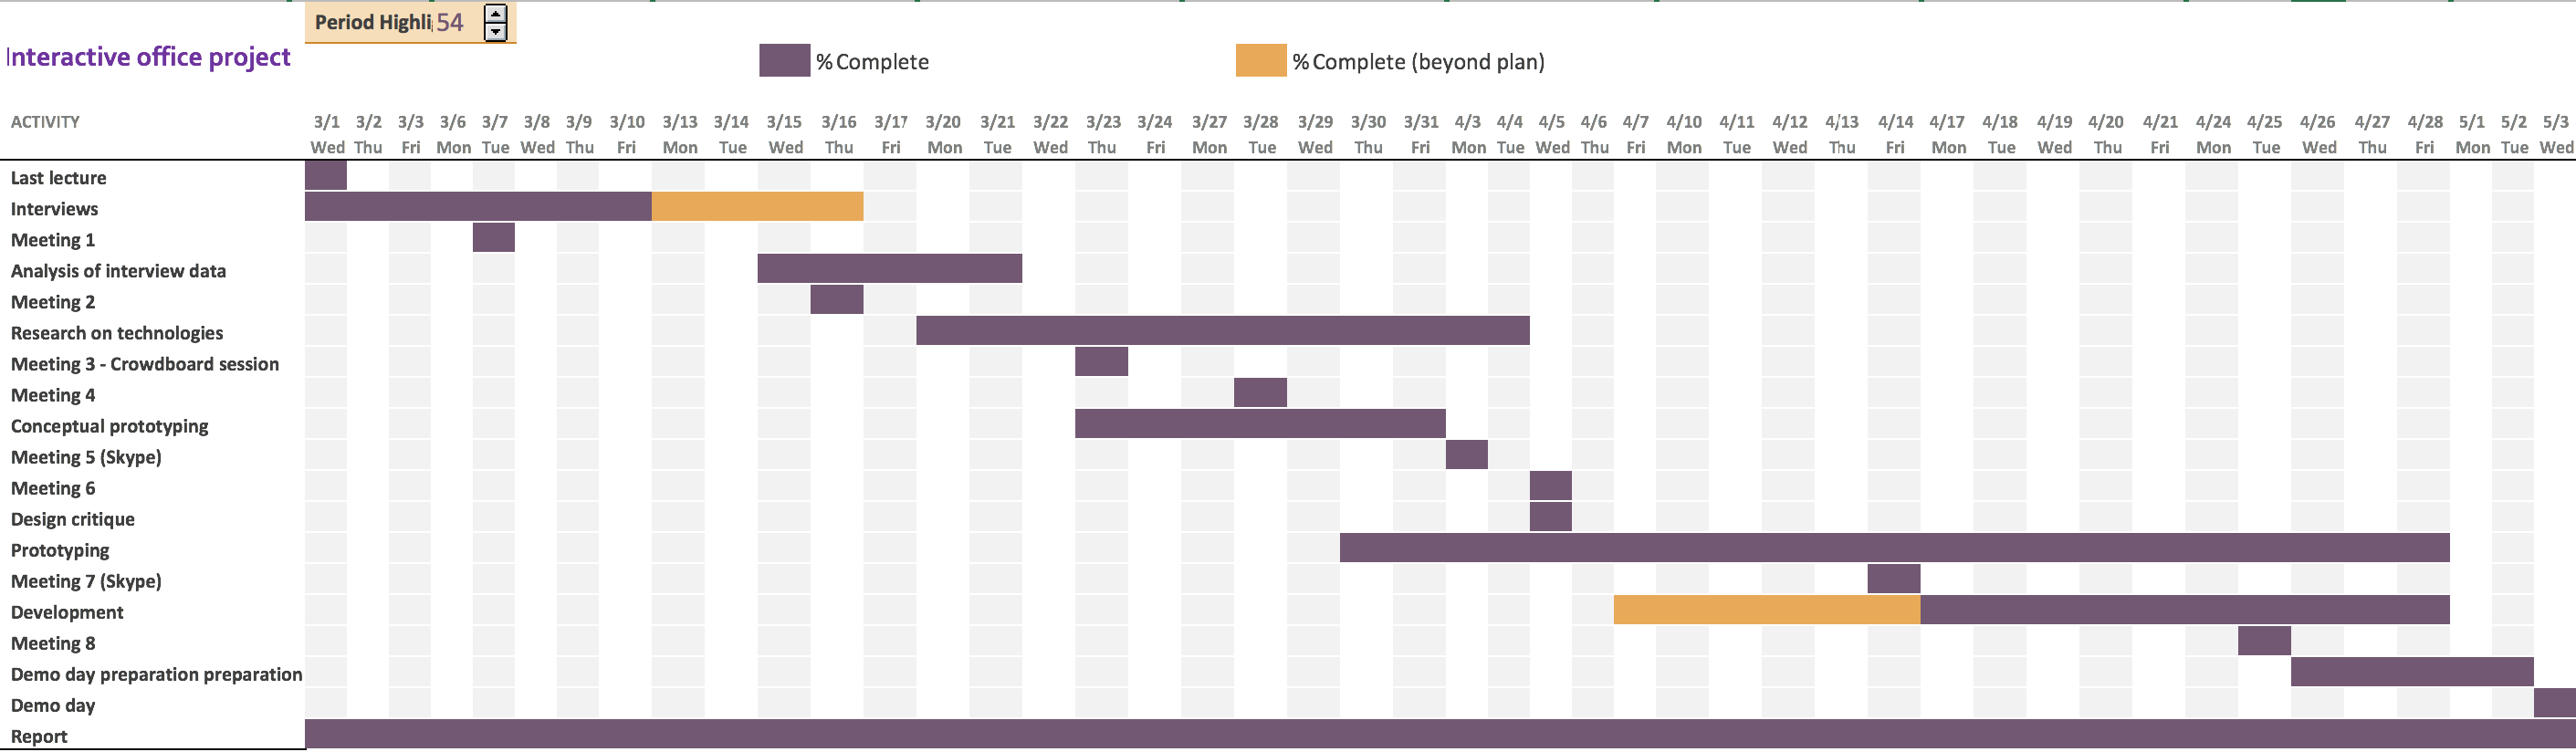
\includegraphics[width=1\textwidth]{images/gantt-chart.png}
			\caption{The Gantt chart of the project.}
			\label{gantt-chart}
		\end{center}
	\end{figure} 
 
% github as a working tool
To make the communication and knowledge sharing among team members, a Facebook group and a Google Drive folder was 
configured. For future source code version tracking, a Github page\footnote{\url{https://github.com/orgs/
InteractiveOfficeProject/}} was configured. The full source code of the project and the report is made available 
through this page for the public. 

For the wireframes and prototype design, Microsoft Visio was used. To design the APIs, a Swagger \footnote{\url{http://swagger.io}} 
page was modified. Project Rider\footnote{\url{https://www.jetbrains.com/rider/}}, a IntelliJ and ReSharper based .NET 
IDE, was used for the client's development.

\subsection{Chosen technologies}
The application is separated into a client and a server application.
% what resources are utilized for carrying the project out? 

% what technologies, development principles are chosen and followed and why? 

%what do we build upon?

\paragraph{Client} It was decided to develop the client in GTK\#. We chose this framework because all of our 
team-members had previous experience with C\#. We also were aware, that GTK\# with Mono is platform-independent -- our 
client should be able to run on Linux, MacOS, and Windows. However, we were unable to build the client in a way that 
it actually runs on all platforms supported by GTK\#; the current releases only run on Linux.

We decided to follow a LEAN\footnote{\url{https://en.wikipedia.org/wiki/Lean_product_development}} approach to create 
a minimum viable product (MVP) and extend this application in small steps to get a running application as soon as 
possible.

A screenshot of the MVP is displayed in Figure \ref{fig:mvp-screenshot}. It has only 2 functionalities: to notify the 
user the user 25 minutes after work has been started and to notify the user 5 minutes after a break has been started. 
Both ``starting work'' and ``starting break'' have to be manually triggered by the users via clicking the 
corresponding buttons. This MVP will then extended step-by-step with the remaining features.

\begin{figure}
  \centering
  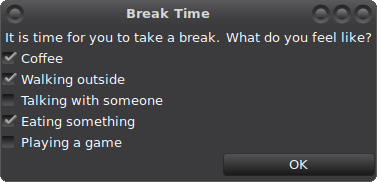
\includegraphics{images/mvp-screenshot.png}
  \caption{Client MVP}
  \label{fig:mvp-screenshot}
\end{figure}

\subparagraph{Future Extensions}
The MVP currently contains only offline functionality. Communication with the server and functions like user matchup were not yet implemented. For demo purposes, there is an example matchup with the authors of this paper. Our next extension points would be to add server communication by priority of the features.

The most important features would be to load the activity list from the server and not use default activities. With 
this, companies could modify the available activities on their locally installed server. The next extension point 
would be to add actual user match-ups. This topic needs some further research. Our current idea is to implement 
so-called break-queues to which the users are added when they start working. 

To create more matches, we add a ``slack'' time of 5 minutes: users that have less than these 5 minutes left until 
break may be interrupted and notified about taking a break early. See Table \ref{tab:break-queues} as an example. Note 
that the slack value was chosen arbitrarily and needs verification.

\begin{table}[ht]
 \centering
 \begin{tabular}{lll}
  \textbf{User} & \textbf{Time until Break} & \textbf{Eligibile for Break} \\
  \hline
  \(u_1\) &  0 min & Yes \\
  \(u_2\) &  3 min & Yes \\
  \(u_3\) &  5 min & Yes \\
  \(u_4\) &  7 min & No \\
  \(u_6\) & 10 min & No \\
  \hline
 \end{tabular}
 \caption{Break-Queue with a slack of 5 minutes. 3 users may be interrupted for break.}
 \label{tab:break-queues}
\end{table}

When a user decides to take a break, we would load the list of eligible users from the server and order them by matching preferences. If no 
users ``within 5 minutes'' are found, we can extend the eligibility time or suggest snoozing or taking a break alone. 


After implementing the server-based activity system and a basic user matching we can further extend the activity 
system. In the first step, only predefined activities are supported. A step to extend this would be to enable users 
suggesting own activities. With this, a whole bunch of new activities could be added to the system without being 
hardcoded. the current system does not have any room information and only suggest some basic activities that should be 
possible in every company, e.g. taking a coffee break or going for a walk. 

Another possible extension point would be to extend the user profiles Currently, the very simple profiles only contain 
the user's name, his/her email address and an optional profile picture. This could be extended by taking the user's 
preferred activities -- thus saving or simplifying the activity selection step -- and the user's preferred working 
schedule\footnote{Currently, work times are 25 minutes long while (short) breaks take 5 minutes as suggested by the 
Pomodoro technique.}. 

A final extension we will look at is taking the surroundings of the company into account. The following may not work 
for all companies as it is based on the locality of the company: we query the Google Maps API for selected location 
types like Cafes, parks, or restaurants. Based on the weather and on the distance to these places we may suggest a 
``walk in the park'' or  ``eating an ice cream in Cafe X''.

\paragraph{Backend}
% flask & python
The technology used for the server component is Flask \footnote{\url{http://flask.pocoo.org/}} and Python \footnote{\url{https://www.python.org/}}. 
Flask is a microframework, which allows easy configuration and debugging of server applications. Getting started with 
the technology is easy, since our team had some expertise in the programming language and we considered it to fit our 
needs perfectly. 

\paragraph{APIs}
The basic APIs were designed among the first components during the development. The APIs development includes the 
definition of the communication protocol channels, models and the possible values that are sent between the client and 
the server in both directions. 

In terms of technology, a traditional RESTful \footnote{\url{https://en.wikipedia.org/wiki/Representational\_state\_transfer}} 
API was chosen and designed. The chosen data format is JSON \footnote{\url{https://en.wikipedia.org/wiki/JSON}} due to 
its simplicity, easiness and wide usage in the present time. 

The APIs are not discussed further and are out of the scope of this document. Nevertheless, the history of the git 
repository and the model's source code is available via the GitHub page \footnote{\url{https://github.com/InteractiveOfficeProject/api-documentation}} 
and the HTML documentation is made public via the department's websites \footnote{\url{http://pivanics.users.cs.helsinki.fi/interactive-office-api-documentation/}}. 